\documentclass[11pt]{article}
\usepackage{graphicx}
\usepackage{hyperref}
\usepackage{natbib}

\setlength{\textwidth}{6.5in}
\setlength{\headheight}{0in}
\setlength{\textheight}{8.0in}
\setlength{\hoffset}{0in}
\setlength{\voffset}{0in}
\setlength{\oddsidemargin}{0in}
\setlength{\evensidemargin}{0in}

\title{PS1: my goal}
  
\author{Shihong Pan}


\begin{document}

\maketitle

\abstract{This document inclues my goal for phys-ga2000, my background in programming and numerics, and my plan after completing the PhD program.}

\section{Main text}
\label{sec:main}

I expect to gain deep understanding of numerical simulation in physics problems after finishing this course. I'm fluent in using numpy and matplotlib due to undergrad research experience, and  I'm familiar with C and C++. I also completed one numerical computation course in undergraduate program. After completing the PhD program, I would probably either find a research job in industries (or national labs), or look for faculty positions in academia.

\section{Github account}

My Github account name is PSH-hub24.


\begin{figure}[b!]
\centering
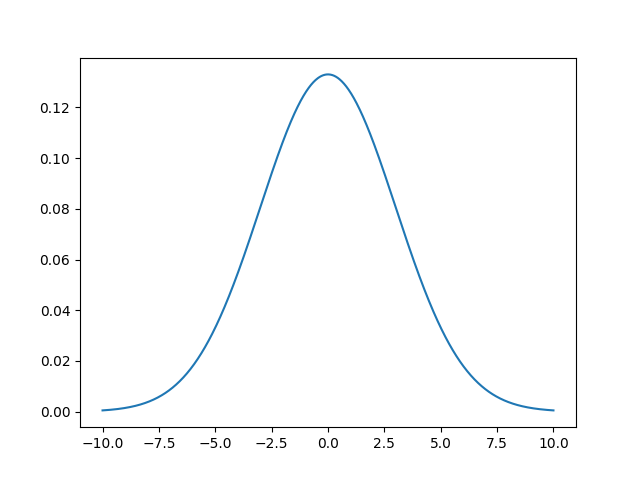
\includegraphics[width=0.95\textwidth]{gaussian.png}
\caption{ \label{fig:example} This is just a plot of a Gaussian with zero mean and a standard deviation of 3 over the range [-10, +10].}
\end{figure}
  

\bibliographystyle{apj}
\bibliography{example}

\end{document}

 
 
